\section{Architettura del prodotto}

\subsection{Descrizione generale}
Il progetto \textit{Predire in Grafana} prevede la realizzazione di due moduli: un plug-in per la piattaforma Grafana e un tool esterno di supporto, rispettivamente chiamati \textbf{Prediction Plug-in} e \textbf{Prediction Tool}. \\
Il Prediction Tool si occupa di addestrare un algoritmo di \textit{SVM} o \textit{Regressione Lineare} utilizzando un dataset inserito dall'utente, per poi generare un file json contenente le informazioni necessarie per poter effettuare un calcolo di predizione. Questo modulo è stato sviluppato seguendo il pattern \textit{Model-View-ViewModel (MVVM)}.\\
Il Prediction Plug-in invece si occuperà di ricevere in input il json e una volta collegati i predittori, contenuti nel file, ad un flusso dati, permetterà di iniziare ad effettuare i calcoli di previsione. Questo modulo è stato sviluppato seguendo il pattern \textit{Model-View-Controller (MVC)}.\\
Le motivazioni principali che hanno portato alla scelta del design pattern MVVM per il Prediction Tool sono:
\begin{itemize}
	\item per la realizzazione del componente è stato utilizzato \textit{React} e abbiamo ritenuto che questo pattern si accoppiasse bene con la struttura di quest'ultimo.
\end{itemize}
Le motivazioni principali che hanno portato alla scelta del design pattern MVC per il Prediction Plug-in sono:
\begin{itemize}
	\item abbiamo ritenuto che questo pattern si accoppiasse meglio con la struttura dei plug-in di Grafana.
\end{itemize}
Inoltre entrambi i pattern permettono:
\begin{itemize}
	\item di disaccoppiare la parte di \textit{presentation logic} da quella di \textit{business logic};
	\item il riutilizzo di alcune componenti in altri contesti, senza doverli modificare.
\end{itemize}
Di seguito sono mostrati i diagrammi delle attività corrispondenti agli Use Cases descritti nell'\textit{Analisi dei Requisiti}.


\subsubsection{Diagrammi delle attività}
\begin{figure}[H]
\centering
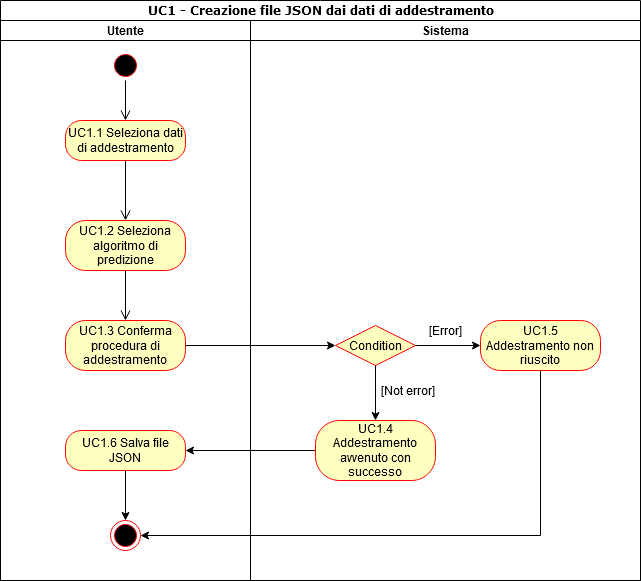
\includegraphics[scale=0.6]{../../Diagrams/Activity_diagrams/uc1.png}
\caption{Diagramma delle attività dello UC1}
\end{figure}
\textbf{Specifica:} lo UC1.5 racchiude i seguenti tipi di errori: 
\begin{itemize}
	\item \textbf{UC7}: Nessun file CSV caricato;
	\item \textbf{UC8}: Nessun algoritmo selezionato;
	\item \textbf{UC9}: File CSV incompatibile.
\end{itemize}
\begin{figure}[H]
\centering
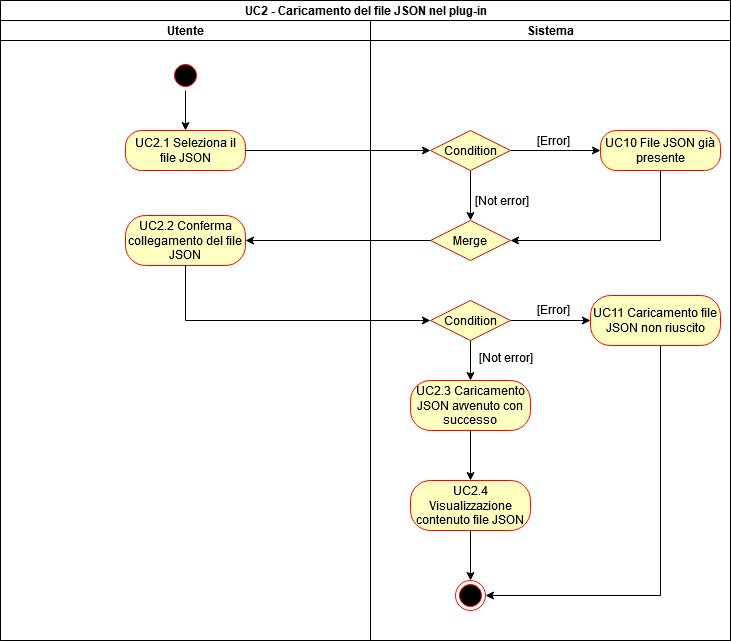
\includegraphics[scale=0.6]{../../Diagrams/Activity_diagrams/uc2.png}
\caption{Diagramma delle attività dello UC2}
\end{figure}
\begin{figure}[H]
\centering
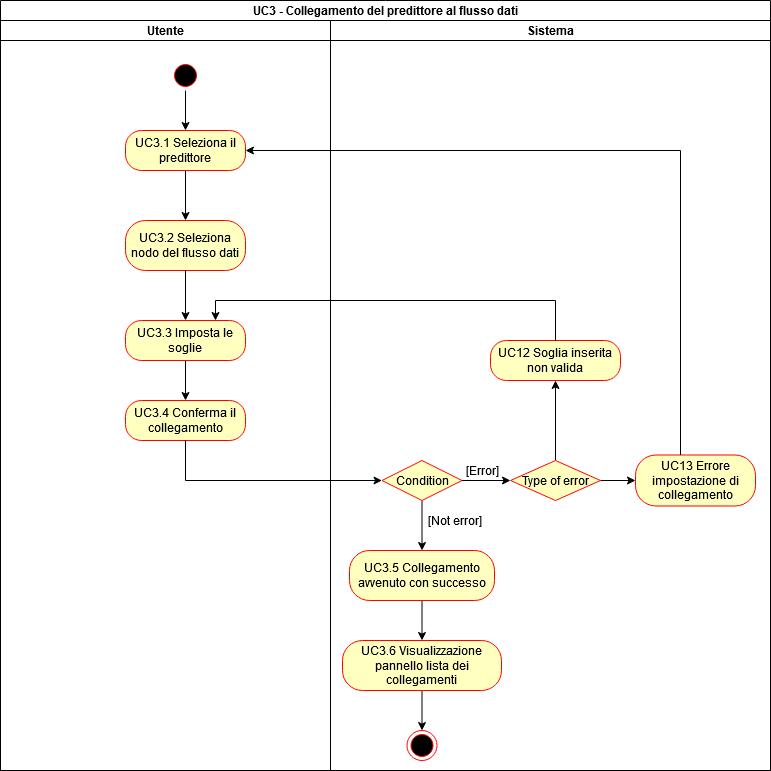
\includegraphics[scale=0.6]{../../Diagrams/Activity_diagrams/uc3.png}
\caption{Diagramma delle attività dello UC3}
\end{figure}
\begin{figure}[H]
\centering
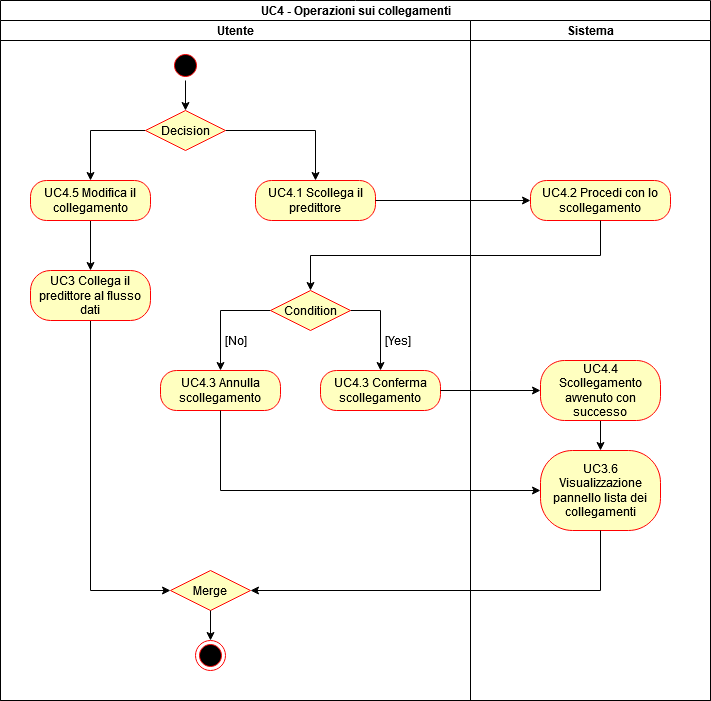
\includegraphics[scale=0.6]{../../Diagrams/Activity_diagrams/uc4.png}
\caption{Diagramma delle attività dello UC4}
\end{figure}
\begin{figure}[H]
\centering
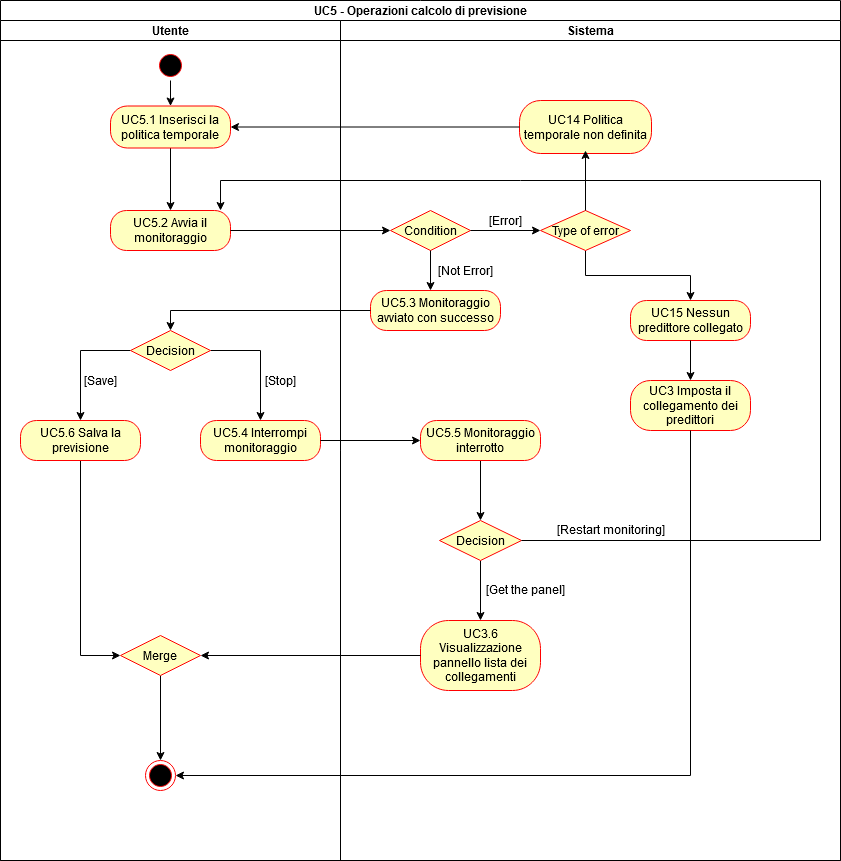
\includegraphics[scale=0.5]{../../Diagrams/Activity_diagrams/uc5.png}
\caption{Diagramma delle attività dello UC5}
\end{figure}
\begin{figure}[H]
\centering
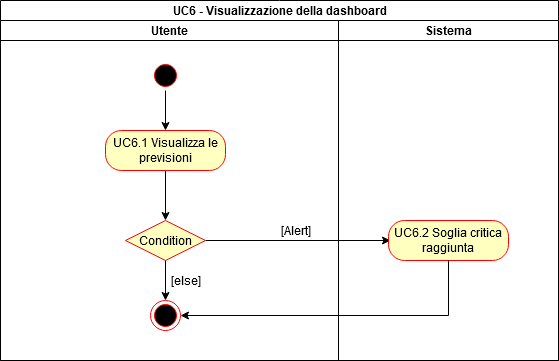
\includegraphics[scale=0.6]{../../Diagrams/Activity_diagrams/uc6.png}
\caption{Diagramma delle attività dello UC6}
\end{figure}

\subsection{Architettura Prediction Tool}

\subsubsection{Descrizione}
L'implemetenazione del tool è stata realizzata utilizzando il design pattern MVVM.
Il passaggio di dati dalle view al model avviene attraverso la modifica di un campo dati \textit{props} immesso dal \textit{ViewModel}.
Attraverso queste \textit{props} il \textit{ViewModel} chiama le funzioni corrette quando l’utente interagisce con la vista.
La divisione tra Business Logic\glo e Presentation Logic è rafforzato da questo utilizzo delle \texttt{props}.
Nel modello viene fornita funzionalità per la gestione degli algoritmi tramite le classi \textit{SVMtrain} e \textit{RLtrain} che verranno utilizzate dal \textit{ViewModel}.


\begin{comment} si trovano un'istanza delle classi SVMtrain e RLtrain in base all'algoritmo scelto, le classi stesse si trovano nel modello e si occupano di rendere polimorfe le funzioni principali, come quelle di addestramento o di recupero del file JSON.
\end{comment}

\subsubsection{Diagrammi dei package}
\begin{figure}[H]
\centering
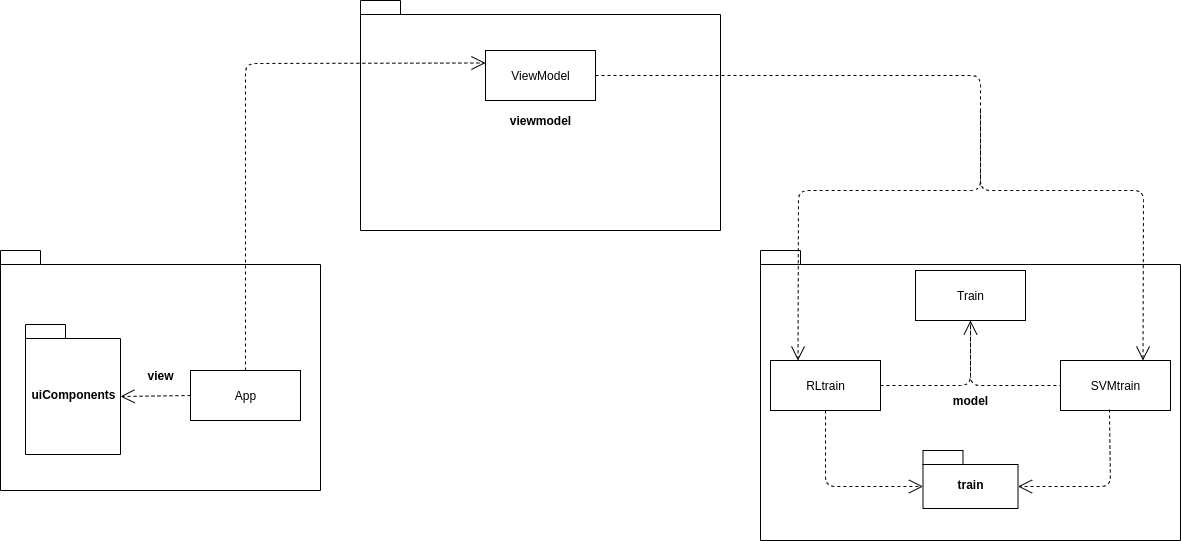
\includegraphics[scale=0.4]{../../Diagrams/Package_diagrams/tool_design_patern.png}
\caption{Diagramma dei package del Prediction Tool}
\end{figure}

\subsubsection{Diagrammi delle classi}
Quello che segue è il diagramma delle classi del Prediction Tool.

\begin{figure}[H]
\centering
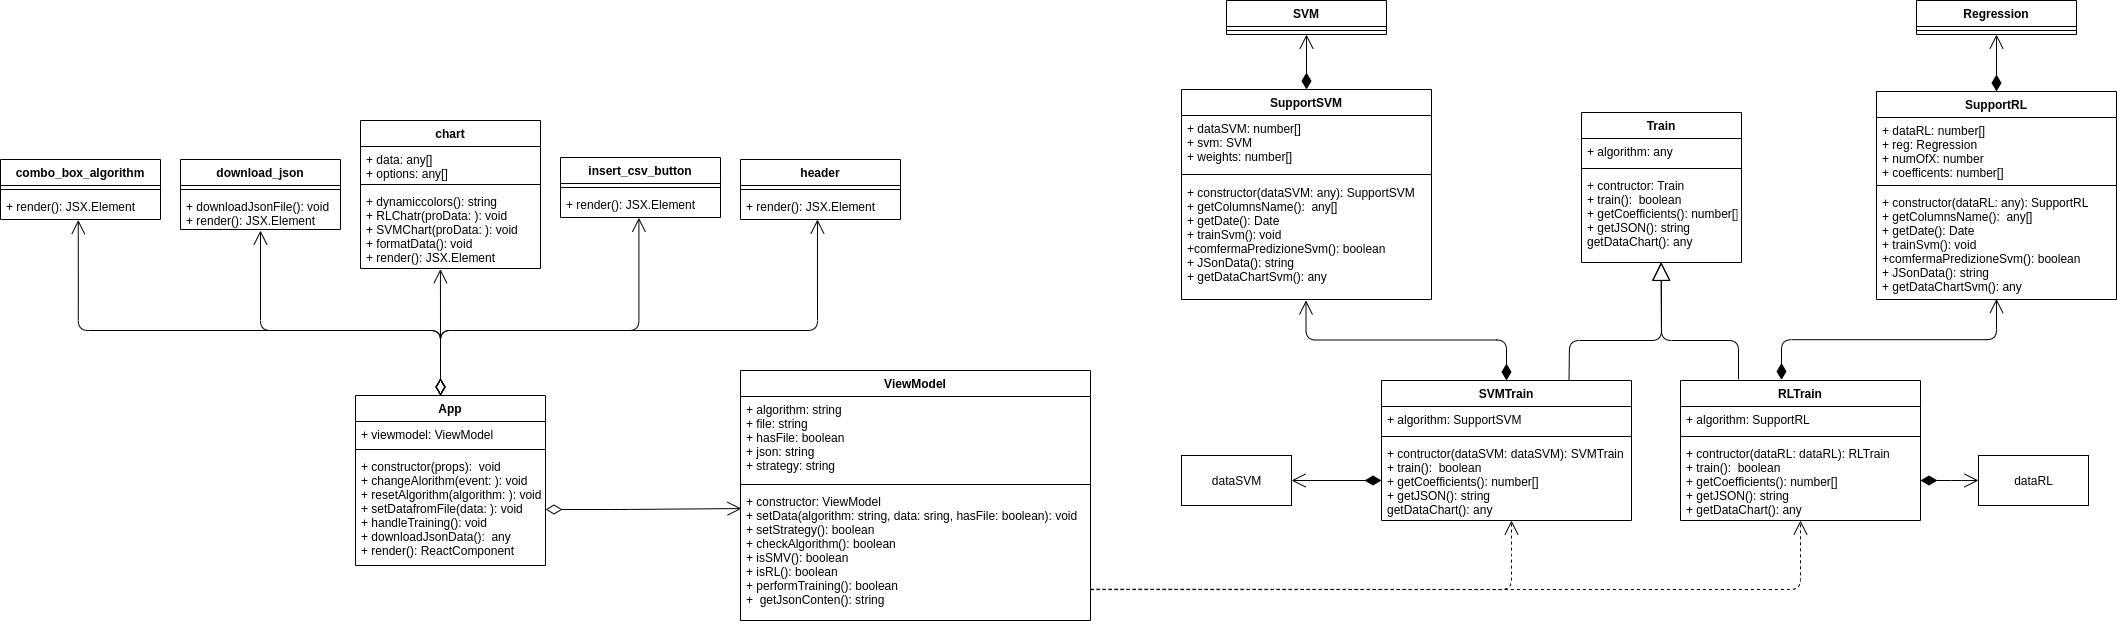
\includegraphics[scale=0.22]{../../Diagrams/Classes_diagrams/tool_all_classes.png}
\caption{Diagramma delle classi del Prediction Tool}
\end{figure}

\begin{comment}
\begin{figure}[H]
\centering
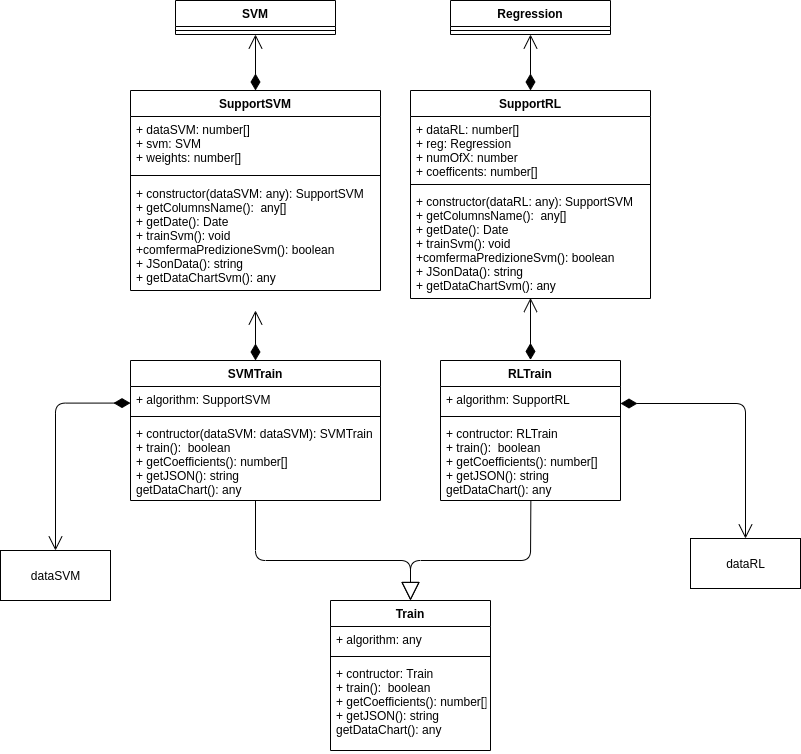
\includegraphics[scale=0.5]{../../Diagrams/Classes_diagrams/tool_model.png}
\caption{Diagramma delle classi del Model del Prediction Tool}
\end{figure}
\pagebreak
\textbf{View}
\begin{figure}[H]
\centering
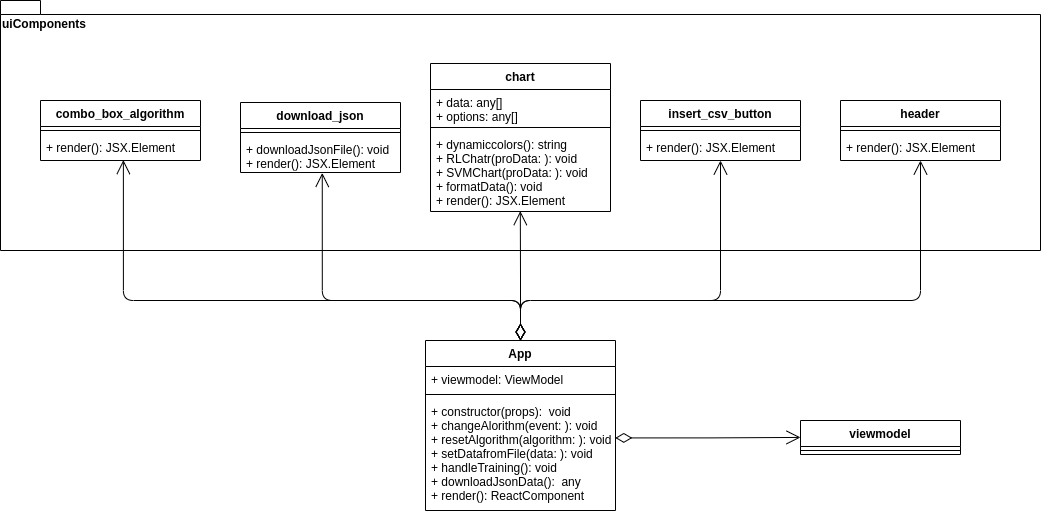
\includegraphics[scale=0.45]{../../Diagrams/Classes_diagrams/tool_view.png}
\caption{Diagramma delle classi della View del Prediction Tool}
\end{figure}

\textbf{ViewModel}
\begin{figure}[H]
\centering
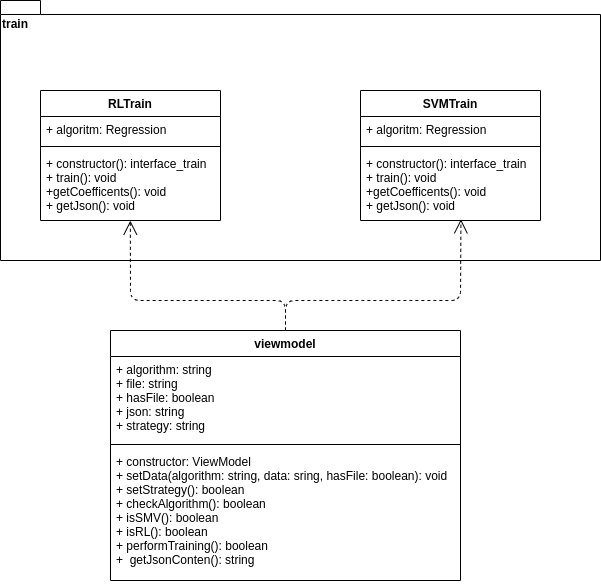
\includegraphics[scale=0.5]{../../Diagrams/Classes_diagrams/tool_modelview.png}
\caption{Diagramma delle classi del ViewModel del Prediction Tool}
\end{figure}
\end{comment}

\subsubsection{Diagrammi di sequenza}
\begin{figure}[H]
\centering
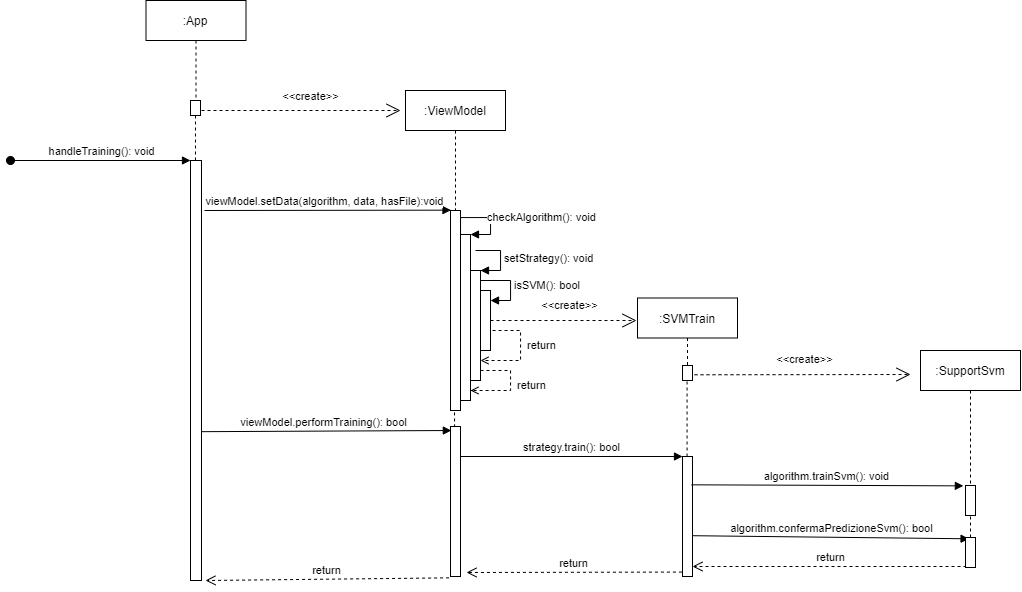
\includegraphics[scale=0.45]{../../Diagrams/Sequence_diagrams/trainSVM.png}
\caption{Diagramma di sequenza del TrainSVM}
\end{figure}

\subsubsection{Design pattern comportamentali utilizzati}
Per quanto riguarda i design pattern comportamentali utilizzati, durante la progettazione delle classi del Prediction Tool ci siamo accorti che alcune classi correlate tra loro (quelle adibite a richiamare le librerie per gli algoritmi di Machine Learning RL e SVM) differivano soltanto per il comportamento effettivo, dato dalla libreria richiamata. I metodi utilizzati dalle due classi erano in effetti più varianti di uno stesso algoritmo (quello di addestramento). Per queste ragioni abbiamo pensato di utilizzare il design pattern \textbf{Strategy}, così da definire una famiglia di algoritmi, incapsularli e renderli interscambiabili tra di loro, a seconda della scelta effettuata dall’utente.
Nel nostro caso abbiamo identificato come \textit{Strategy} l’oggetto contenente un riferimento all'algoritmo di previsione.
Quest'ultimo rappresenta il modello della nostra applicazione, dove è contenuta effettivamente la business logic.

\pagebreak
\subsection{Architettura Prediction Plug-in}

\subsubsection{Descrizione}
In questo modulo, composto da più pannelli all'interno di Grafana, verrà associato il predittore prodotto dal tool esterno al flusso dati monitorato appunto in Grafana. Per questo modulo è stato utilizzato il pattern architetturale \textit{MVC}.
In questa architettura l’Editor e il Panel condividono la variabile \textit{props}, istanziata da Grafana. 
All’importazione del file JSON, il controller si occuperà di: \begin{itemize}
\item leggere il suo contenuto attraverso la funzione \texttt{setJson(file)};
\item salvare una copia dei predittori;
\item applicare l'algoritmo di previsione corretto attraverso il metodo \texttt{setStrategy()};
\item inviare una notifica alla viste di successo caricamento file JSON.
\end{itemize}
\begin{comment}
\textbf{AGGIUNGERE RIGUARDO MODEL E VIEW}
\end{comment}
Per quanto riguarda la comunicazione che avviene tra \textit{View} e \textit{Model} viene gestita dal \textit{Controller}. Questo è stato reso possibile per la presenza in \textit{Editor} di un istanza della classe \textit{Controller}. In questo modo, ad ogni caricamento del file JSON, il \textit{Controller} viene messo al corrente dal pannello \textit{CaricamentoJsonView} (tramite il metodo \textbf{update()}) di aggiornare gli oggetti del modello ed inviare i le nuove informazioni alla vista.


A seguito di una discussione col proponente, abbiamo deciso di creare una componente Panel come punto di partenza del nostro plug-in, la quale ha il compito di creare una dashboard per permettere all’utente di prendere familiarità con le funzionalità dei vari pannelli.

\subsubsection{Diagrammi dei package}
\begin{figure}[H]
\centering
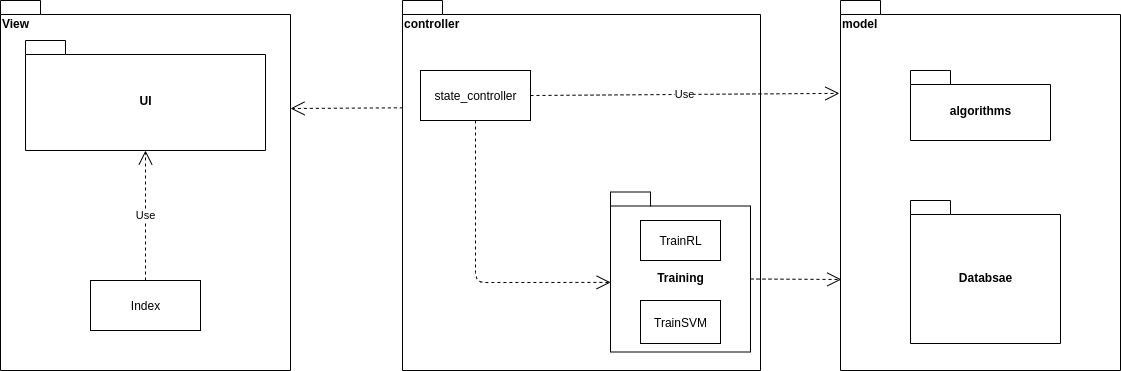
\includegraphics[scale=0.40]{../../Diagrams/Package_diagrams/plugin_design_pattern.png}
\caption{Diagramma dei package del Prediction Plug-in}
\end{figure}

\subsubsection{Diagrammi delle classi}
\textbf{Model}
\begin{figure}[H]
\centering
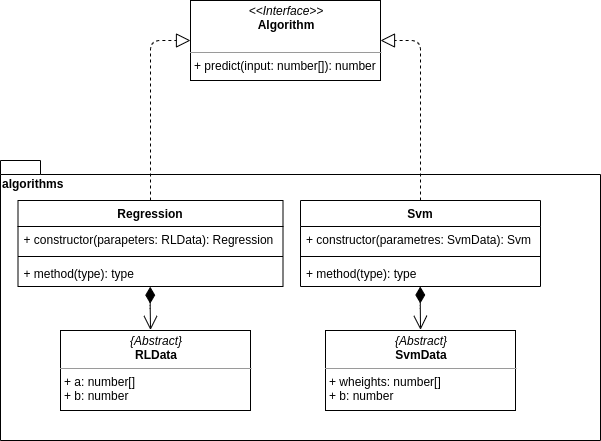
\includegraphics[scale=0.45]{../../Diagrams/Classes_diagrams/plugin_model.png}
\caption{Diagramma delle classi del Model del Prediction Plug-in}
\end{figure}

\textbf{View}
\begin{figure}[H]
\centering
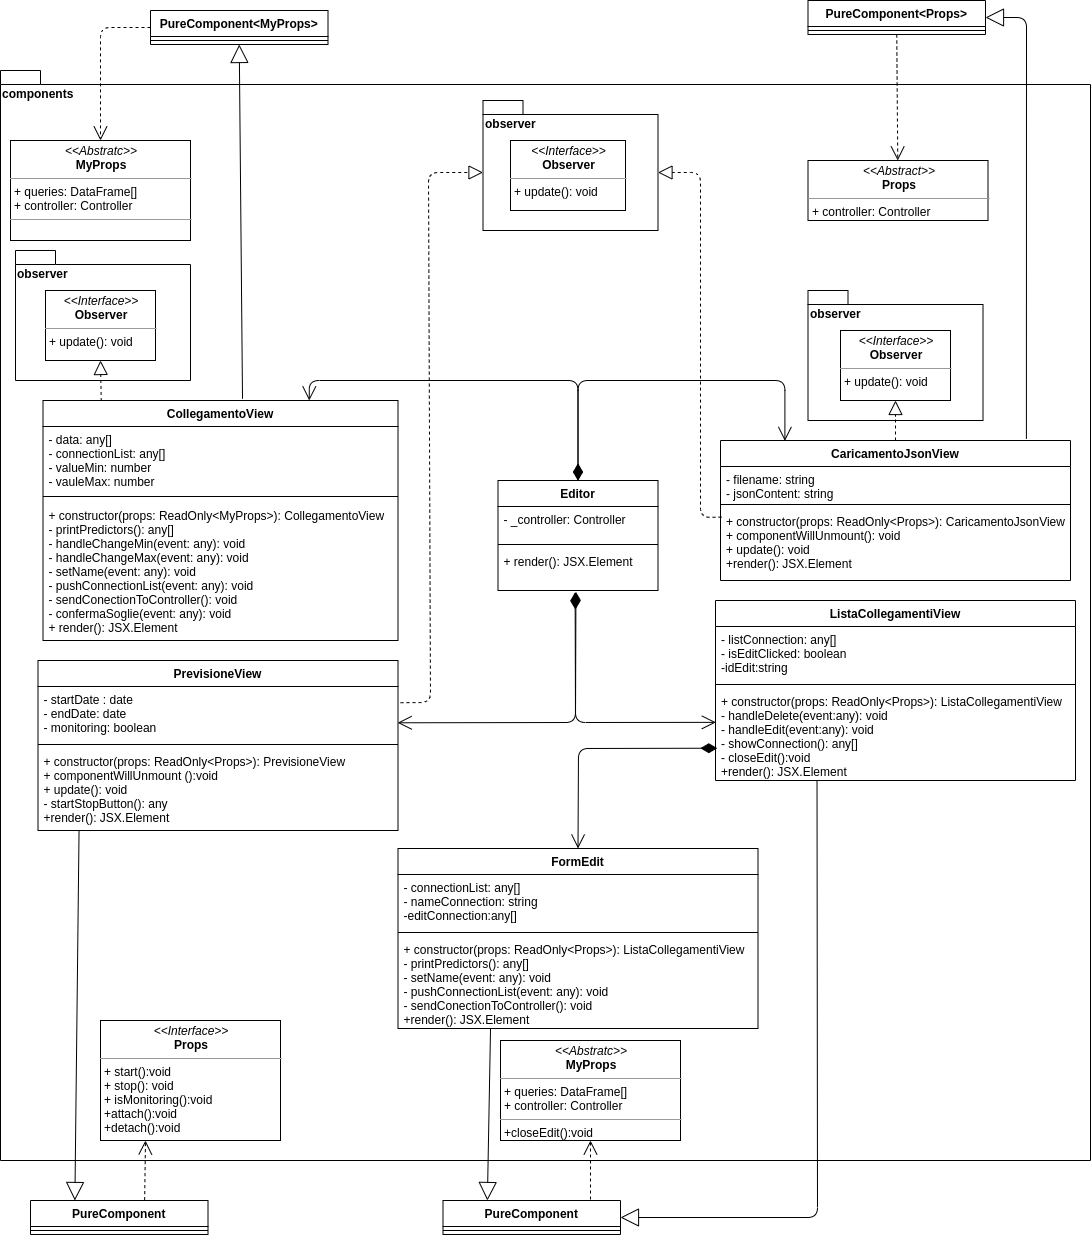
\includegraphics[scale=0.4]{../../Diagrams/Classes_diagrams/plugin_view.png}
\caption{Diagramma delle classi della View del Prediction Plug-in}
\end{figure}

\textbf{Controller}
\begin{figure}[H]
\centering
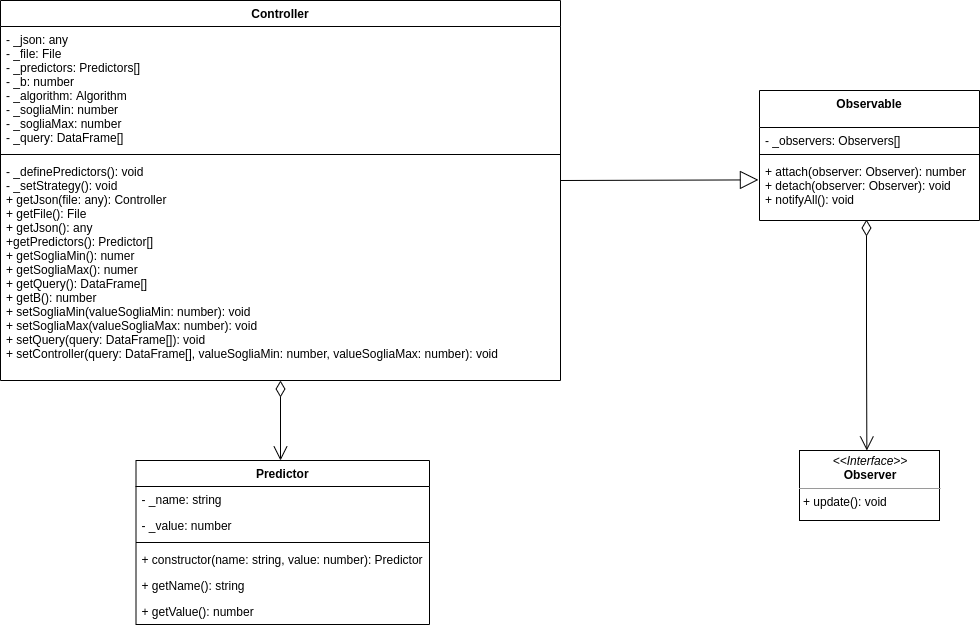
\includegraphics[scale=0.4]{../../Diagrams/Classes_diagrams/plugin_controller.png}
\caption{Diagramma delle classi del Controller del Prediction Plug-in}
\end{figure}

\subsubsection{Diagrammi di sequenza}

\subsubsection{Design pattern comportamentali utilizzati}
Tra i design pattern notevoli che sono stati adottati per l'implementazione del plugin, rientra l'\textbf{Observer Pattern} il quale dà la possibiltà di garantire l'aggiornamento dei componenti in seguito a modifiche da parte dell'utente.
Nel nostro caso la classe \textit{subject}, ovvero le classi da monitorare sono tutte le componenti grafiche utilizzate dalla classe \textit{Editor}. Invece la l'interfaccia \textit{Observe}, implementata dalla \textit{Observable}, è colei che ha il compito di segnalare la necessità di un aggiornamento delle componenti del plugin.

